\documentclass[]{article}
\usepackage{lmodern}
\usepackage{amssymb,amsmath}
\usepackage{ifxetex,ifluatex}
\usepackage{fixltx2e} % provides \textsubscript
\ifnum 0\ifxetex 1\fi\ifluatex 1\fi=0 % if pdftex
  \usepackage[T1]{fontenc}
  \usepackage[utf8]{inputenc}
\else % if luatex or xelatex
  \ifxetex
    \usepackage{mathspec}
    \usepackage{xltxtra,xunicode}
  \else
    \usepackage{fontspec}
  \fi
  \defaultfontfeatures{Mapping=tex-text,Scale=MatchLowercase}
  \newcommand{\euro}{€}
\fi
% use upquote if available, for straight quotes in verbatim environments
\IfFileExists{upquote.sty}{\usepackage{upquote}}{}
% use microtype if available
\IfFileExists{microtype.sty}{%
\usepackage{microtype}
\UseMicrotypeSet[protrusion]{basicmath} % disable protrusion for tt fonts
}{}
\ifxetex
  \usepackage[setpagesize=false, % page size defined by xetex
              unicode=false, % unicode breaks when used with xetex
              xetex]{hyperref}
\else
  \usepackage[unicode=true]{hyperref}
\fi
\hypersetup{breaklinks=true,
            bookmarks=true,
            pdfauthor={Eric Anderson},
            pdftitle={Metworx 3.1.0},
            colorlinks=true,
            citecolor=blue,
            urlcolor=blue,
            linkcolor=magenta,
            pdfborder={0 0 0}}
\urlstyle{same}  % don't use monospace font for urls
%%%\setlength{\parskip}{6pt plus 2pt minus 1pt}
\setlength{\emergencystretch}{3em}  % prevent overfull lines
\providecommand{\tightlist}{%
  \setlength{\itemsep}{0pt}\setlength{\parskip}{0pt}}
\setcounter{secnumdepth}{5}

%%% Use protect on footnotes to avoid problems with footnotes in titles
\let\rmarkdownfootnote\footnote%
\def\footnote{\protect\rmarkdownfootnote}

%%% Change title format to be more compact
\usepackage{titling}

% Create subtitle command for use in maketitle
\newcommand{\subtitle}[1]{
  \posttitle{
    \begin{center}\large#1\end{center}
    }
}

\setlength{\droptitle}{-2em}
  \title{Metworx 3.1.0}
  \pretitle{\vspace{\droptitle}\centering\huge}
  \posttitle{\par}
  \author{Eric Anderson}
  \preauthor{\centering\large\emph}
  \postauthor{\par}
  \predate{\centering\large\emph}
  \postdate{\par}
  \date{September 11, 2017}

\usepackage{pdfpages}
\usepackage{pdflscape}
\usepackage{graphicx}
\usepackage{geometry}
\usepackage{bm}
\usepackage{multirow}
\newcommand{\figDir}{../deliv/figure}
\newcommand{\tabDir}{../deliv/table}
\usepackage{longtable}
\usepackage{fancyhdr, lastpage}
\usepackage{caption}
\usepackage{subcaption}

\pagestyle{fancy}

% http://stackoverflow.com/a/27334272
\newcommand{\blandscape}{\begin{landscape}}
\newcommand{\elandscape}{\end{landscape}}


\usepackage{textpos}
\usepackage{float}
\floatplacement{figure}{H}
\floatplacement{table}{H}


\newcommand{\metworx}{Metworx\texttrademark}

\newcommand{\proptitle}{CR: METWORX AMI v3.0.1}
\newcommand{\topic}{Extend \metworx\ to include NONMEM 7.4}

\newcommand{\testinglogTwelve}{ami-metworx-3-0-1intel12.pdf}
\newcommand{\testinglogFourteen}{ami-metworx-3-0-1intel14.pdf}
\newcommand{\propversion}{metworx-3.0.1}




\usepackage{pdfpages}

% Redefines (sub)paragraphs to behave more like sections
\ifx\paragraph\undefined\else
\let\oldparagraph\paragraph
\renewcommand{\paragraph}[1]{\oldparagraph{#1}\mbox{}}
\fi
\ifx\subparagraph\undefined\else
\let\oldsubparagraph\subparagraph
\renewcommand{\subparagraph}[1]{\oldsubparagraph{#1}\mbox{}}
\fi

%%%%%%%%change date format to metrum style%%%%%%%
\usepackage{datetime}
\newcommand{\todaymetrum}{\the\year-\twodigit{\month}-\twodigit{\day}}

\usepackage{fancyhdr, lastpage}

\pagestyle{fancy}

\rhead{Project Number:\  \\Sponsor: }
\lhead{Metrum Research Group LLC\\CONFIDENTIAL}
%\rfoot{Right bottom}
%\cfoot{Page \thepage\ of \pageref{LastPage}}


\usepackage{graphicx}
\usepackage{longtable}
%better control of float; adds [H] option (to be used instead of clearpage in figures/tables sections)
\usepackage{float}
\floatplacement{figure}{H}
\floatplacement{table}{H}
\usepackage{bm}

% \newcommand{\figDir}{../deliv/figure}
% \newcommand{\tabDir}{../deliv/table}
\newcommand{\doctitle}{Metworx 3.1.0}

\newcommand{\clientname}{Client Name}
\newcommand{\clienttitle}{Client Title}
\newcommand{\companyname}{Company Name}
\newcommand{\clientstreet}{123 Street Rd.}
\newcommand{\clientcitystate}{City, State ZIP}
\newcommand{\clientcountry}{Country}
\newcommand{\clientphone}{Phone: 555-555-5555}
\newcommand{\clientfax}{Fax: 555-555-5554}
\newcommand{\clientemail}{name@domain.com}

\newcommand{\scientist}{Eric Anderson}
\newcommand{\scientistphone}{Phone: 860-735-7043}
\newcommand{\scientistfax}{Fax: 860-760-6014}


\rhead{Project Number:CR-56  \\Sponsor:Metrum RG }
\lhead{Metrum Research Group LLC\\CONFIDENTIAL}
%\rfoot{Right bottom}
%\cfoot{Page \thepage\ of \pageref{LastPage}}


\begin{document}
%\maketitle
\setlength{\parindent}{0pt}


\vspace*{1cm}
\begin{center}
{\large CONFIDENTIAL}


\vspace*{1cm}


\vspace*{1cm}

{\huge CR-56: Metworx 3.1.0}
\vspace{3.0cm}

\begin{tabular}{|p{7cm}|p{7cm}|}\hline
Submitted to: & Author:\\\hline
Jeffrey T. Hane & Eric Anderson \\
Metrum Research Group LLC & Metrum Research Group LLC\\
  & 2 Tunxis Road, Suite 112\\
  & Tariffville, CT\\
  & Email: \href{mailto:andersone@metrumrg.com}{\nolinkurl{andersone@metrumrg.com}}  \\\hline

  Initiator Submitted to QA   & \\

  & \\
  & \\
  & \\\hline

  IS Review   & \\

  & \\
  & \\
  & \\\hline
  
  Scientific Review   & \\

  & \\
  & \\
  & \\\hline


QA Approval  & \\

 & \\
 & \\
 & \\\hline

 Assigned CR Number: & \\

 & \\
 & \\
 & \\\hline


\end{tabular}

\end{center}


\newpage



\section{Definitions}\label{definitions}

\textbf{Amazon Machine Image (AMI):} A virtual machine template for all
instances launched within Metworx

\textbf{Chef:} Software for scripted, reproducible hardware abstraction
(\url{https://www.chef.io/})

\textbf{Cookbook:} The unit of code (Ruby) within Chef that dictates
configuration of specific software or functionality

\textbf{Git:} Version control software used by MetrumRG with relation to
infrastructure source code control

\textbf{Metworx:} Metrum Research Group's pharmacometric modeling
platform for use with Amazon Web Services (AWS)

\textbf{metrumrg R package:} A collection of R functions which assist in
pharmacometric modeling and other Metrum Research Group essential
activities (\url{https://r-forge.r-project.org/projects/metrumrg/})

\textbf{Envision Index:} Web application for Envision developers and
users to access and configure Envision Apps.

\section{Purpose}\label{purpose}

To validate newly created Envision Index, which will be the new landing
page when users go to Envision. \vspace{1cm}

\begin{figure}
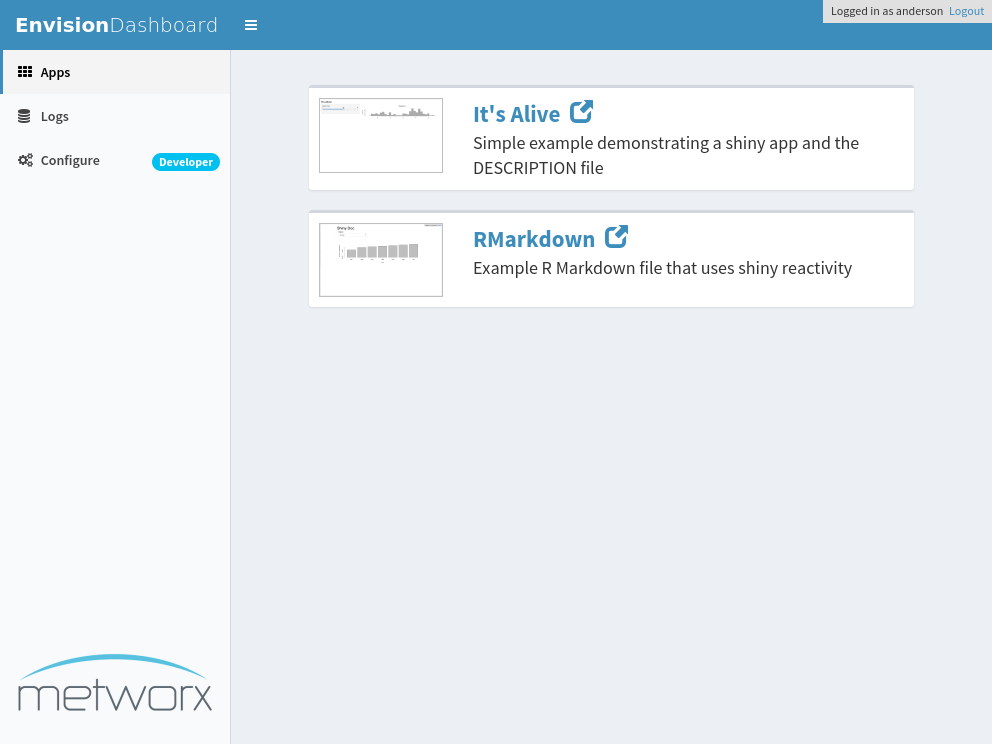
\includegraphics[width=428px,height=321px]{Envision-Index-Testing_files/figure-latex/unnamed-chunk-2-1} \caption{Envsion Index Testing}\label{fig:unnamed-chunk-2}
\end{figure}\begin{figure}
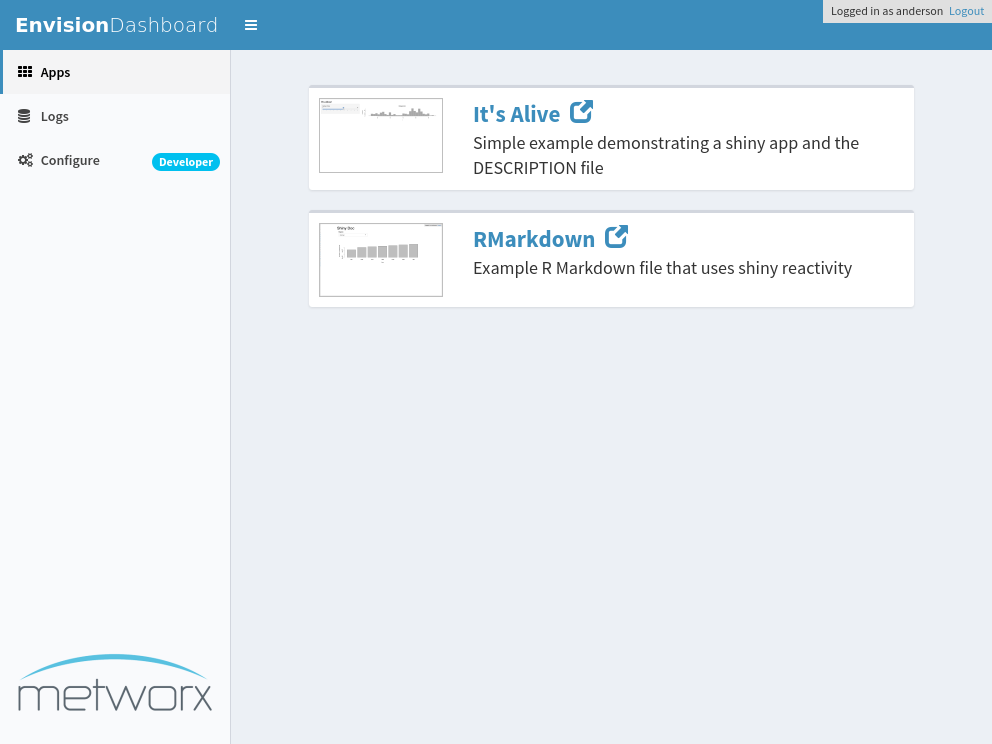
\includegraphics[width=428px,height=321px]{Envision-Index-Testing_files/figure-latex/unnamed-chunk-2-2} \caption{Envsion Index Testing}\label{fig:unnamed-chunk-2}
\end{figure}

\end{document}
